\documentclass{article}

\usepackage{graphicx}
\usepackage{verbatim}

\author{Mohammad Afroz Alam}
\date{}
\title{CV Assignment 3 Readme}
\begin{document}

\section{Time Taken}
\begin{itemize}
\item Time taken for conv1 = 0.000958919525146 secs
\item Time taken for conv2 = 0.00978302955627 secs
\item Time taken for conv3 = 0.00294518470764 secs
\item Time taken for conv4 = 0.00292491912842 secs
\item Time taken for conv5 = 0.0381109714508 secs
\item Time taken for fc1 = 0.000120878219604 secs
\item Time taken for fc2 = 0.000124216079712 secs
\end{itemize}

\section{Number of Parameters}
\begin{itemize}
\item Conv 1 : 155
\item Conv 2 : 2416
\item Fc 1 : 48120
\item Fc 2 : 10164
\item Fc 3 : 850
\end{itemize}

\section{t-SNE plots}
\begin{figure}[h]
  \centering
  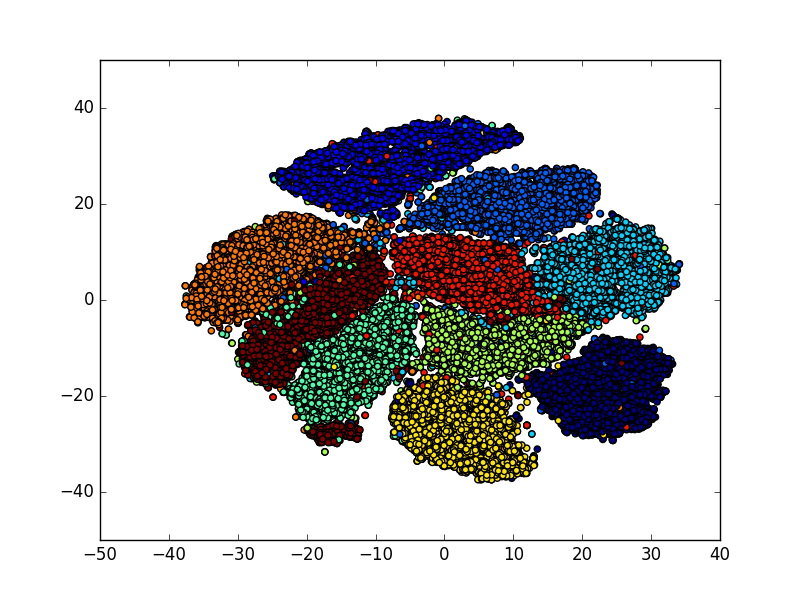
\includegraphics[width=0.7\textwidth]{keras_lenet/scatter_basic.png}
  \caption{Without 84 dimensional features for 50000 images}
  \label{fig:basic}
\end{figure}

\begin{figure}[h]
  \centering
  \includegraphics[width=0.7\textwidth]{keras_lenet/scatter_encoding.png}
  \caption{With 84 dimensional features for 10000 images(Keras)}
\end{figure}

\begin{figure}[h]
  \centering
  \includegraphics[width=0.7\textwidth]{scatter_encoding.png}
  \caption{With 84 dimensional features for 10000 images (My Implementation)}
\end{figure}

\section{Training and Validation Losses}

\begin{figure}[h]
  \centering
  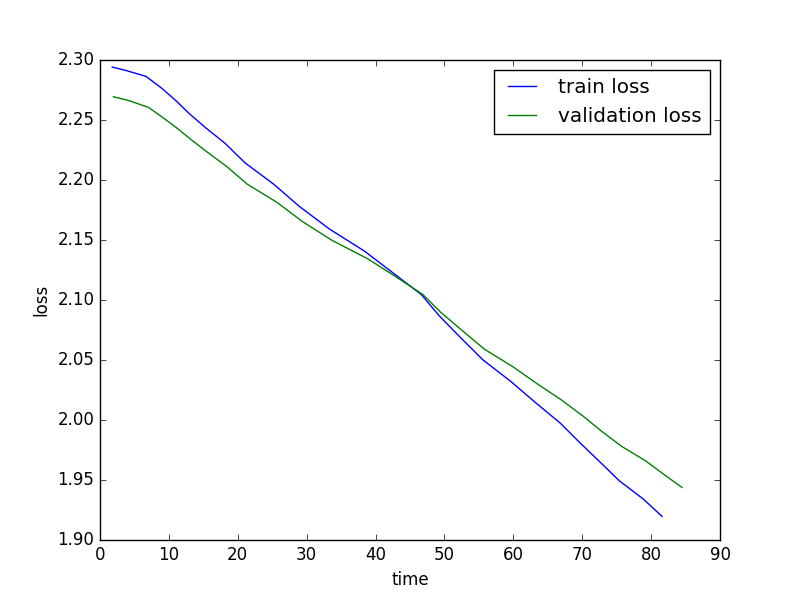
\includegraphics[width=0.7\textwidth]{loss.png}
  \caption{Train and Validation loss for batch size 160 (My Implementation)}
\end{figure}

\begin{figure}[h]
  \centering
  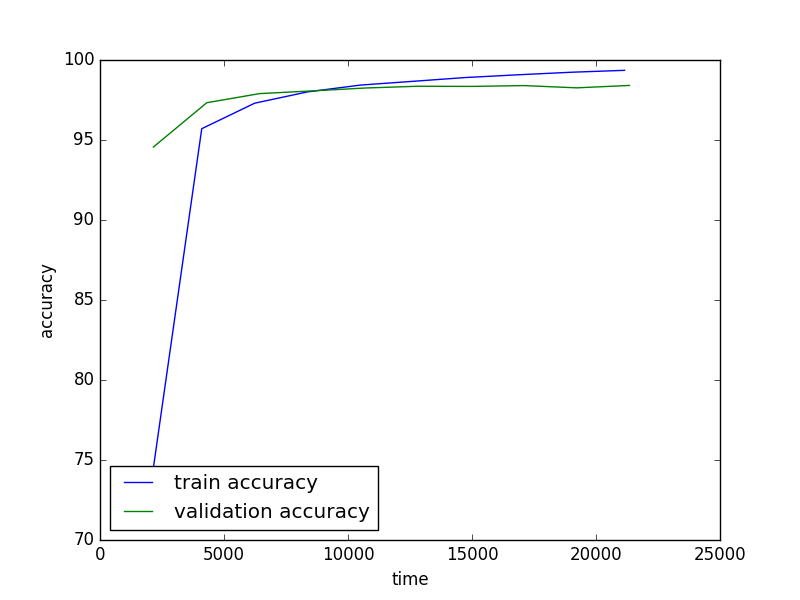
\includegraphics[width=0.7\textwidth]{accuracy.png}
  \caption{Train and Validation accuracy for batch size 160 (My Implementation)}
\end{figure}

\begin{figure}[h]
  \centering
  \includegraphics[width=\textwidth]{keras_lenet/acc_epoch.png}
  \caption{Accuracy on different batch sizes per epoch (Keras)}
\end{figure}

\begin{figure}[h]
  \centering
  \includegraphics[width=\textwidth]{keras_lenet/acc_time.png}
  \caption{Accuracy on different batch sizes per time (Keras)}
\end{figure}

\begin{figure}[h]
  \centering
  \includegraphics[width=\textwidth]{keras_lenet/loss_epoch.png}
  \caption{Loss on different batch sizes per epoch (Keras)}
\end{figure}

\begin{figure}[h]
  \centering
  \includegraphics[width=\textwidth]{keras_lenet/loss_time.png}
  \caption{Loss on different batch sizes per epoch (Keras)}
\end{figure}

\subsection{Conclusion}
The training converges fastest with batch size 64 when we observe the
loss and accuracy with respect to time.
\end{document}

%%% Local Variables:
%%% mode: latex
%%% TeX-master: t
%%% End:
